% Shared preamble for the CIG-AMF formal-research papers.
% IEEEtran conference class; compiles on Overleaf without modification.
\documentclass[conference]{IEEEtran}
\IEEEoverridecommandlockouts

\usepackage{cite}
\usepackage{amsmath,amssymb,amsfonts}
\usepackage{amsthm}
\usepackage{algorithm}
\usepackage{algorithmic}
\usepackage{graphicx}
\usepackage{textcomp}
\usepackage{xcolor}
\usepackage{booktabs}
\usepackage{url}
\usepackage[hidelinks]{hyperref}

\def\BibTeX{{\rm B\kern-.05em{\sc i\kern-.025em b}\kern-.08em T\kern-.1667em\lower.7ex\hbox{E}\kern-.125emX}}

\newtheorem{theorem}{Theorem}
\newtheorem{lemma}[theorem]{Lemma}
\newtheorem{proposition}[theorem]{Proposition}
\newtheorem{corollary}[theorem]{Corollary}
\theoremstyle{definition}
\newtheorem{definition}[theorem]{Definition}
\newtheorem{remark}[theorem]{Remark}
\newtheorem{example}[theorem]{Example}

% A machine-checked statement carries its Lean declaration name.
\newcommand{\lean}[1]{\textsf{\footnotesize #1}}
\newcommand{\leanbox}[1]{%
  \par\vspace{2pt}\noindent
  {\footnotesize\textsf{Lean: #1}}\par\vspace{2pt}}

% Evidence classes, used consistently and never interchangeably.
\newcommand{\PROVED}{\textsc{proved}}
\newcommand{\CERT}{\textsc{certificate}}
\newcommand{\NUM}{\textsc{numerical}}
\graphicspath{{../_figures/}}


\begin{document}

\title{Deciding Without Identifying:\\
An Equivariant Decoder That Is Minimax Over\\
All Decision Rules}

\author{\IEEEauthorblockN{Vu Phan An Nguyen}
\IEEEauthorblockA{\textit{Rider University} \\
Lawrenceville, NJ, USA}}

\maketitle

\begin{abstract}
A class contains $a$ safe tips and $b$ unsafe tips in a finite set $T$. A world is the
unsafe set $W\subseteq T$ with $|W|=b$; observations reveal only unsafe tips, so a
transcript is a revealed subset $R\subseteq W$. The task is to \emph{name a safe tip}, not
to identify $W$. Identifying the world is a coupon-collector problem whose cost grows with
the number of classes $K$; naming a safe tip need not be, and we determine exactly how much
cheaper deciding is and whether the natural decoder---name a tip drawn uniformly from the
unexplored set---is optimal or merely convenient. We prove five things. The number of unsafe
tips still hidden is the same for every world compatible with a transcript, so the decoder's
conditional risk is a function of the transcript alone: equivariance is proved, not assumed,
and the risk equals $L/(a+L)$ with $L=b-|R|$. Bayes risk factors through a posterior loss,
the pointwise-argmin rule is optimal over \emph{all} rules, and such a rule exists because
the action set is finite---so the infimum is attained and no limiting argument is needed.
Chaining these, the equivariant decoder is a \emph{least element} of the achievable
worst-case risks, which closes a real gap: the earlier statement took constant risk as a
hypothesis and contained no infimum over rules, so it said the decoder was flat, not that it
was optimal. Flatness is itself discharged from symmetry rather than imposed. Finally the
decide risk is exactly $\tfrac12(1-P)^{N}$, independent of $K$, while recovery grows like
$K\log K$: the separation is an identity, not an asymptotic comparison. Each displayed theorem is machine-checked in Lean~4 with no \texttt{sorry}; Section~\ref{sec:verification} names the steps the paper works out itself.
\end{abstract}

\begin{IEEEkeywords}
decision theory, minimax risk, Bayes risk, active learning, equivariance,
formal verification, interactive theorem proving
\end{IEEEkeywords}

\section{Introduction}

Suppose a finite set $T$ of tips contains $a$ safe ones and $b$ unsafe ones. The world is
the unsafe set $W\subseteq T$ with $|W|=b$. Observations are destructive in the sense that
they reveal only unsafe tips: a transcript is a revealed subset $R\subseteq W$, and nothing
in the transcript distinguishes between the ways the remaining $b-|R|$ unsafe tips could be
distributed among the tips not yet seen.

The task is to name a safe tip. It is \emph{not} to identify $W$, and that distinction is
the subject of the paper.

\subsection{Where the problem comes from}

The abstraction above describes a recurring situation. A maintenance crew inspects
components and a failed inspection identifies a bad component but a passed one is not
recorded; a security team probes endpoints and only vulnerable ones respond; a screening
process flags positives and is silent on negatives. In each case the transcript accumulates
evidence of one kind only, and the operational question is not what the full state is but
which single item is safe to use, deploy, or release.

The asymmetry in the observation process is what makes the problem interesting rather than
trivial. If both safe and unsafe tips were revealed, a transcript of size $|R|$ would pin
down $|R|$ tips exactly and the decision would be immediate whenever any safe tip had been
seen. Because only unsafe tips appear, the transcript never directly exhibits a safe tip,
and the decoder must always name an item it has no direct evidence about.

That is also why the equivariance of Section~\ref{sec:decoder} is not obvious in advance.
The decoder names an unexplored tip, and the unexplored set is the part of $T$ about which
the transcript is silent; one might expect its composition to vary across compatible worlds.
Lemma~\ref{lem:hidden} says it does not, and that single counting fact is what the rest of
the argument is built on.

\subsection{Why the distinction matters}

Identifying the world is a coupon-collector problem: across $K$ classes, one must see enough
of each to pin down its unsafe set, and the cost grows with $K$. Naming a safe tip need not
be: a decision is correct as soon as the named tip happens to be safe, whether or not the
world is known.

Two questions follow. How much cheaper is deciding than recovering---and is the answer an
asymptotic comparison or an exact one? And is the natural decoder, which names a tip drawn
uniformly from the unexplored set, actually optimal, or merely the obvious thing to do?

\subsection{The gap this paper closes}

An earlier treatment of this problem lifted a Bayes bound to a worst case for the natural
decoder. That statement took constant risk as a \emph{hypothesis} and contained no infimum
over rules. It therefore said the decoder was \emph{flat}---its risk does not vary with the
world---and said nothing about whether any other rule does better. Flatness is a property of
the decoder; optimality is a property of the problem, and the two are independent: a rule
can be perfectly flat and uniformly terrible.

Closing the gap requires three things the earlier statement lacked: a form in which an
arbitrary rule's contribution separates observation by observation, a proof that the
pointwise minimiser is optimal over all rules, and a proof that such a minimiser exists.
Sections~\ref{sec:bayes} and \ref{sec:minimax} supply them, and the flatness hypothesis is
discharged from symmetry rather than imposed.

\subsection{Contributions}

\begin{enumerate}
\item[C1.] \textbf{A decoder whose risk is a function of the transcript alone.} The number of
unsafe tips still hidden is the same for every world compatible with the transcript
(Lemma~\ref{lem:hidden}), so the conditional risk depends on the transcript and not on the
world (Theorem~\ref{thm:equivariant}). Equivariance is proved, not assumed.

\item[C2.] \textbf{Minimaxity over all decision rules.} Bayes risk factors through a
posterior loss (Theorem~\ref{thm:factor}), the pointwise-argmin rule is optimal over all
rules and exists (Theorem~\ref{thm:optimal}), and hence the equivariant decoder is a least
element of the achievable worst-case risks (Theorem~\ref{thm:minimax}).

\item[C3.] \textbf{Flatness from symmetry rather than assumption.} A risk invariant under a
transitive relabelling of worlds is constant (Proposition~\ref{prop:symmetry}).

\item[C4.] \textbf{An exact decide--recover separation, flat in $K$.} The decide risk is
exactly $\tfrac12(1-P)^{N}$, independent of $K$, while recovery grows like $K\log K$
(Theorem~\ref{thm:separation}). The separation is an identity, not an asymptotic comparison.

\item[C5.] \textbf{The sampling law, exactly.} The probability that a tuple goes unseen is
$(1-s)^{N}$ by a product law, and the expectation of a product of indicators factors as
$B(1-s)^{N}$ by exchanging two finite sums (Theorem~\ref{thm:sampling}).
\end{enumerate}

\subsection{Roadmap}

Section~\ref{sec:setting} fixes notation and Section~\ref{sec:related} the novelty boundary.
Section~\ref{sec:sampling} gives the sampling law and Section~\ref{sec:decoder} the decoder
and its equivariance. Sections~\ref{sec:bayes} and \ref{sec:minimax} build the minimax
chain, and Section~\ref{sec:chain} sets out what each of its four links contributes and
which one was absent before. Section~\ref{sec:separation} gives the decide--recover
separation, Section~\ref{sec:results} the exact counts, Section~\ref{sec:worked} a small
instance carried through the whole argument, Section~\ref{sec:verification} the formal
development, and Section~\ref{sec:discussion} the scope.

A reader interested only in the closed gap can read Sections~\ref{sec:bayes},
\ref{sec:minimax} and \ref{sec:chain}; one interested only in the separation can read
Sections~\ref{sec:sampling}, \ref{sec:separation} and \ref{sec:results}. The two halves
share the model and the decoder but are otherwise independent.

\section{Setting and notation}
\label{sec:setting}

\begin{table}[htbp]
\caption{Notation.}
\label{tab:notation}
\centering
\footnotesize
\begin{tabular}{@{}ll@{}}
\toprule
Symbol & Meaning \\
\midrule
$T$ & the finite set of tips \\
$a$ & number of safe tips \\
$b$ & number of unsafe tips \\
$W$ & the world, $W\subseteq T$ with $|W|=b$ \\
$R$ & the transcript, $R\subseteq W$ \\
$L$ & unsafe tips still hidden, $L=b-|R|$ \\
$r$ & decoder risk, \eqref{eq:decoder} \\
$K$ & number of classes \\
$N$ & number of draws \\
$s,P$ & per-draw probabilities \\
$\pi$ & a prior over worlds \\
$d$ & a decision rule, observation $\mapsto$ action \\
$L(w,a)$ & loss of action $a$ in world $w$ \\
$P(w,x)$ & probability of observation $x$ in world $w$ \\
$g(x,a)$ & posterior loss, \eqref{eq:bayes} \\
$B(d)$ & Bayes risk of rule $d$ \\
$R(w,d)$ & risk of rule $d$ in world $w$ \\
\bottomrule
\end{tabular}
\end{table}

A \emph{decision rule} is any map from observations to actions. Nothing in the development
restricts rules to be deterministic, non-adaptive or measurable in any non-trivial sense:
the observation and action sets are finite, so every map is a rule. This matters for
Theorem~\ref{thm:minimax}, whose force comes from the breadth of the quantifier.

\section{Related work and the novelty boundary}
\label{sec:related}

\subsection{Decision-making versus identification}

Javdani et al.\ \cite{javdani2014} formulate near-optimal Bayesian active learning for
decision making and make exactly the distinction this paper's title names: the goal is to
choose well, not to learn the hypothesis. Their guarantees are approximation ratios for
greedy policies under adaptive submodularity, and they are about the \emph{policy}---how to
choose the next observation---rather than about the decoder that acts on a completed
transcript.

The present paper is complementary and narrower. The observation process here is given, not
designed; what is analysed is the terminal decision, and the result is an exact minimax
statement rather than an approximation ratio. Nothing here improves on
\cite{javdani2014}'s policy guarantees, and nothing there implies
Theorem~\ref{thm:minimax}, which concerns a different object.

\subsection{Minimax decision theory}

The chain Bayes-risk $\to$ posterior loss $\to$ pointwise minimisation $\to$ minimax lower
bound is textbook \cite{lehmann1998}, and Theorems~\ref{thm:factor} and \ref{thm:optimal}
are instances of it. They are proved here rather than cited for two reasons. The formal
development needs them as Lean statements about this problem's finite structures, and---more
substantively---the step that was missing from the earlier treatment is exactly
Theorem~\ref{thm:optimal}, so writing it out is the point rather than a preliminary.

The statement obtained is minimaxity \emph{through one Bayes prior}: a single prior whose
Bayes-optimal risk equals the equivariant decoder's constant risk. This is a standard route
to minimaxity and it is weaker than a general minimax theorem; Section~\ref{sec:discussion}
says so explicitly and no saddle point is claimed.

\subsection{Summary of the boundary}

Claimed as new: the equivariance proof for this decoder (C1); the completion of the minimax
chain for this problem, in particular the infimum over all rules (C2); the discharge of the
flatness hypothesis from symmetry (C3); and the exact decide--recover separation with the
decide side independent of $K$ (C4, C5). The decision-theoretic machinery and the
decision-making-versus-identification framing are cited.

\section{The observation model}
\label{sec:model}

The results are stated against a specific observation process, and stating it precisely
avoids two ambiguities that would otherwise make the theorems hard to apply.

\subsection{What a draw does}

A draw selects a tip according to the model's per-tip probabilities and reports it only if
it is unsafe. Safe tips therefore generate no record: a transcript $R$ after $N$ draws is
the set of unsafe tips that happened to be selected, and the number of draws is not
recoverable from the transcript. Two consequences follow.

First, $|R|$ is a random variable with $|R|\le b$ always, and the transcript saturates once
every unsafe tip has been seen. After saturation further draws are uninformative, which is
why the decide risk \eqref{eq:decide} has the form it does: the event driving it is whether
saturation has occurred, not how many draws were spent.

Second, the analysis of Sections~\ref{sec:decoder}--\ref{sec:minimax} conditions on the
transcript rather than on the draw count. This is deliberate: a decoder sees $R$ and not
$N$, so a risk expressed in terms of $N$ would not be implementable, and
Theorem~\ref{thm:equivariant} gives the risk as a function of $|R|$ precisely so that the
decoder can evaluate it.

\subsection{Across classes}

With $K$ classes, each carries its own safe/unsafe split and its own tips, and a draw
selects within the whole population. The symmetric model of
Section~\ref{sec:separation} takes $a_{i}=b_{i}=1$ per class and $p_{i}=P/K$, so the total
unsafe mass $P$ is held fixed as $K$ grows---which is the comparison that makes the
separation meaningful. Letting $P$ grow with $K$ would make both costs grow and would
confound the question being asked.

Nothing in the cross-class setup assumes independence between classes. The sampling law of
Section~\ref{sec:sampling} uses linearity of expectation, and the recovery law uses
inclusion--exclusion; both are identities on the joint law, whatever it is.

\section{The sampling law}
\label{sec:sampling}

\begin{theorem}[Product law and its expectation]
\label{thm:sampling}
The probability that a given tuple goes unseen in $N$ draws is $(1-s)^{N}$, where $s$ is its
per-draw probability, and the expectation of the product of unseen indicators over a family
of $B$ tuples is $B(1-s)^{N}$.
\end{theorem}

\begin{proof}
The per-draw avoidance probability is computed by a product over the finite index set, which
gives $(1-s)$ per draw and $(1-s)^{N}$ over $N$ independent draws. For the expectation,
exchange the sum over tuples with the sum over draws: the exchange is between two finite
sums and is therefore exact. Note that no independence between classes is assumed anywhere;
linearity of expectation suffices, which is why the result is an identity rather than an
approximation.
\end{proof}

\leanbox{\lean{avoid\_prob}, \lean{prod\_unseen\_card}, \lean{expected\_prod\_unseen} in
\lean{LeanSupportSamplingLawV1}}

\section{The decoder and its risk}
\label{sec:decoder}

\begin{lemma}[The hidden count is world-free]
\label{lem:hidden}
Every world compatible with a transcript $R$ has exactly $b$ unsafe tips and contains all of
$R$. Hence the number of unsafe tips still hidden is $L=b-|R|$ in all of them.
\end{lemma}

\begin{proof}
Compatibility means $R\subseteq W$ and $|W|=b$. The hidden count is $|W\setminus R|$, which
equals $|W|-|R|=b-|R|$ because $R\subseteq W$.
\end{proof}

\leanbox{\lean{hidden\_count\_world\_free} in \lean{LeanSupportEquivariantDecoderV1}}

\begin{theorem}[Equivariance and the closed-form risk]
\label{thm:equivariant}
The decoder that names a tip drawn uniformly from the unexplored set has conditional risk
\begin{equation}
r\;=\;\frac{b-|R|}{a+b-|R|}\;=\;\frac{L}{a+L},
\qquad L=b-|R|,
\label{eq:decoder}
\end{equation}
which depends on the transcript alone and not on the world.
\end{theorem}

\begin{proof}
The unexplored set has $a+b-|R|$ elements, of which $L=b-|R|$ are unsafe by
Lemma~\ref{lem:hidden}. Drawing uniformly, the probability of naming an unsafe tip is the
ratio, which is \eqref{eq:decoder}. Both numerator and denominator are functions of $|R|$,
so the risk is a function of the transcript.
\end{proof}

\leanbox{\lean{decoder\_risk\_world\_free}, \lean{decoder\_risk\_eq\_L\_over\_aL} in
\lean{LeanSupportEquivariantDecoderV1}}

Equivariance is thus a cardinality computation, not an assumption. It is worth noting how
little it uses: only that compatibility forces $R\subseteq W$ and $|W|=b$. Any observation
process with those two properties gives the same conclusion, whatever its dynamics.

\section{Bayes risk factors}
\label{sec:bayes}

Optimality over all rules cannot be argued rule by rule. It needs a form in which a rule's
contribution separates observation by observation.

\begin{theorem}[Factorisation]
\label{thm:factor}
\begin{align}
B(d)&\;=\;\sum_{x} g\bigl(x,\,d(x)\bigr),\notag\\
g(x,a)&\;=\;\sum_{w}\pi(w)\,P(w,x)\,L(w,a).
\label{eq:bayes}
\end{align}
\end{theorem}

\begin{proof}
Write the Bayes risk as $\sum_{w}\pi(w)\sum_{x}P(w,x)L(w,d(x))$ and exchange the two finite
sums. Collecting the rule's action at each observation gives \eqref{eq:bayes}. Both sums are
finite, so the exchange is exact.
\end{proof}

\leanbox{\lean{bayesRisk\_eq\_sum\_postLoss} in \lean{LeanSupportMinimaxLowerV1}}

After Theorem~\ref{thm:factor} the rule appears only inside $g$, once per observation. That
is the entire purpose of the step: the Bayes risk of an arbitrary rule is now a sum of
independent terms, each depending on the rule through a single action.

\section{Optimality over all rules}
\label{sec:minimax}

\begin{theorem}[The pointwise minimum is optimal and attained]
\label{thm:optimal}
\begin{equation}
\sum_{x}\;\min_{a}\;g(x,a)\;\;\leq\;\;B(d)
\qquad\text{for every rule } d,
\label{eq:optimal}
\end{equation}
and the bound is attained by any rule choosing an argmin at every observation. Such a rule
exists because the action set is finite and non-empty.
\end{theorem}

\begin{proof}
By Theorem~\ref{thm:factor}, $B(d)=\sum_{x}g(x,d(x))$, and each summand is at least
$\min_{a}g(x,a)$; summing gives \eqref{eq:optimal}. For attainment, define $d^{*}(x)$ to be
an argmin of $g(x,\cdot)$, which exists as the action set is finite and non-empty. Then
$B(d^{*})=\sum_{x}\min_{a}g(x,a)$.
\end{proof}

\leanbox{\lean{bayes\_optimal\_lower}, \lean{bayes\_optimal\_attained} in
\lean{LeanSupportMinimaxLowerV1}}

The infimum over rules is therefore a \emph{minimum}, and no limiting argument is required.
This is the step the earlier treatment lacked, and it is the reason the conclusion can be
stated as a least element rather than as an infimum that might not be achieved.

\begin{theorem}[Minimax lower bound]
\label{thm:minimax}
\begin{equation}
\sum_{x}\min_{a}g(x,a)\;\;\leq\;\;\sup_{w}R(w,d)
\label{eq:minimax}
\end{equation}
for every rule $d$ and every prior $\pi$. Consequently a rule whose risk is constant and
equal to that number is a least element of the achievable worst-case risks.
\end{theorem}

\begin{proof}
Two inequalities composed. The worst case dominates the Bayes risk for every prior,
$B(d)\le\sup_{w}R(w,d)$, since a weighted average is at most a supremum. Chaining with
\eqref{eq:optimal} gives \eqref{eq:minimax}. If a rule has constant risk equal to the
left-hand side, it achieves that worst case, and by \eqref{eq:minimax} no rule achieves
less.
\end{proof}

\leanbox{\lean{minimax\_ge\_bayes\_optimal}, \lean{equivariant\_is\_minimax} in
\lean{LeanSupportMinimaxLowerV1}}

\begin{proposition}[Flatness from symmetry]
\label{prop:symmetry}
A risk invariant under a transitive relabelling of worlds is constant.
\end{proposition}

\begin{proof}
Transitivity supplies, for any two worlds, a relabelling carrying one to the other;
invariance then equates their risks.
\end{proof}

\leanbox{\lean{constant\_risk\_of\_symmetry} in \lean{LeanSupportMinimaxLowerV1}}

Proposition~\ref{prop:symmetry} is how the constant-risk hypothesis is discharged rather
than imposed. Combined with Theorem~\ref{thm:equivariant}---which gives invariance, since a
risk depending only on $|R|$ is unchanged by relabelling---it yields constancy, and
Theorem~\ref{thm:minimax} then yields optimality.

\begin{figure}[htbp]
\centering
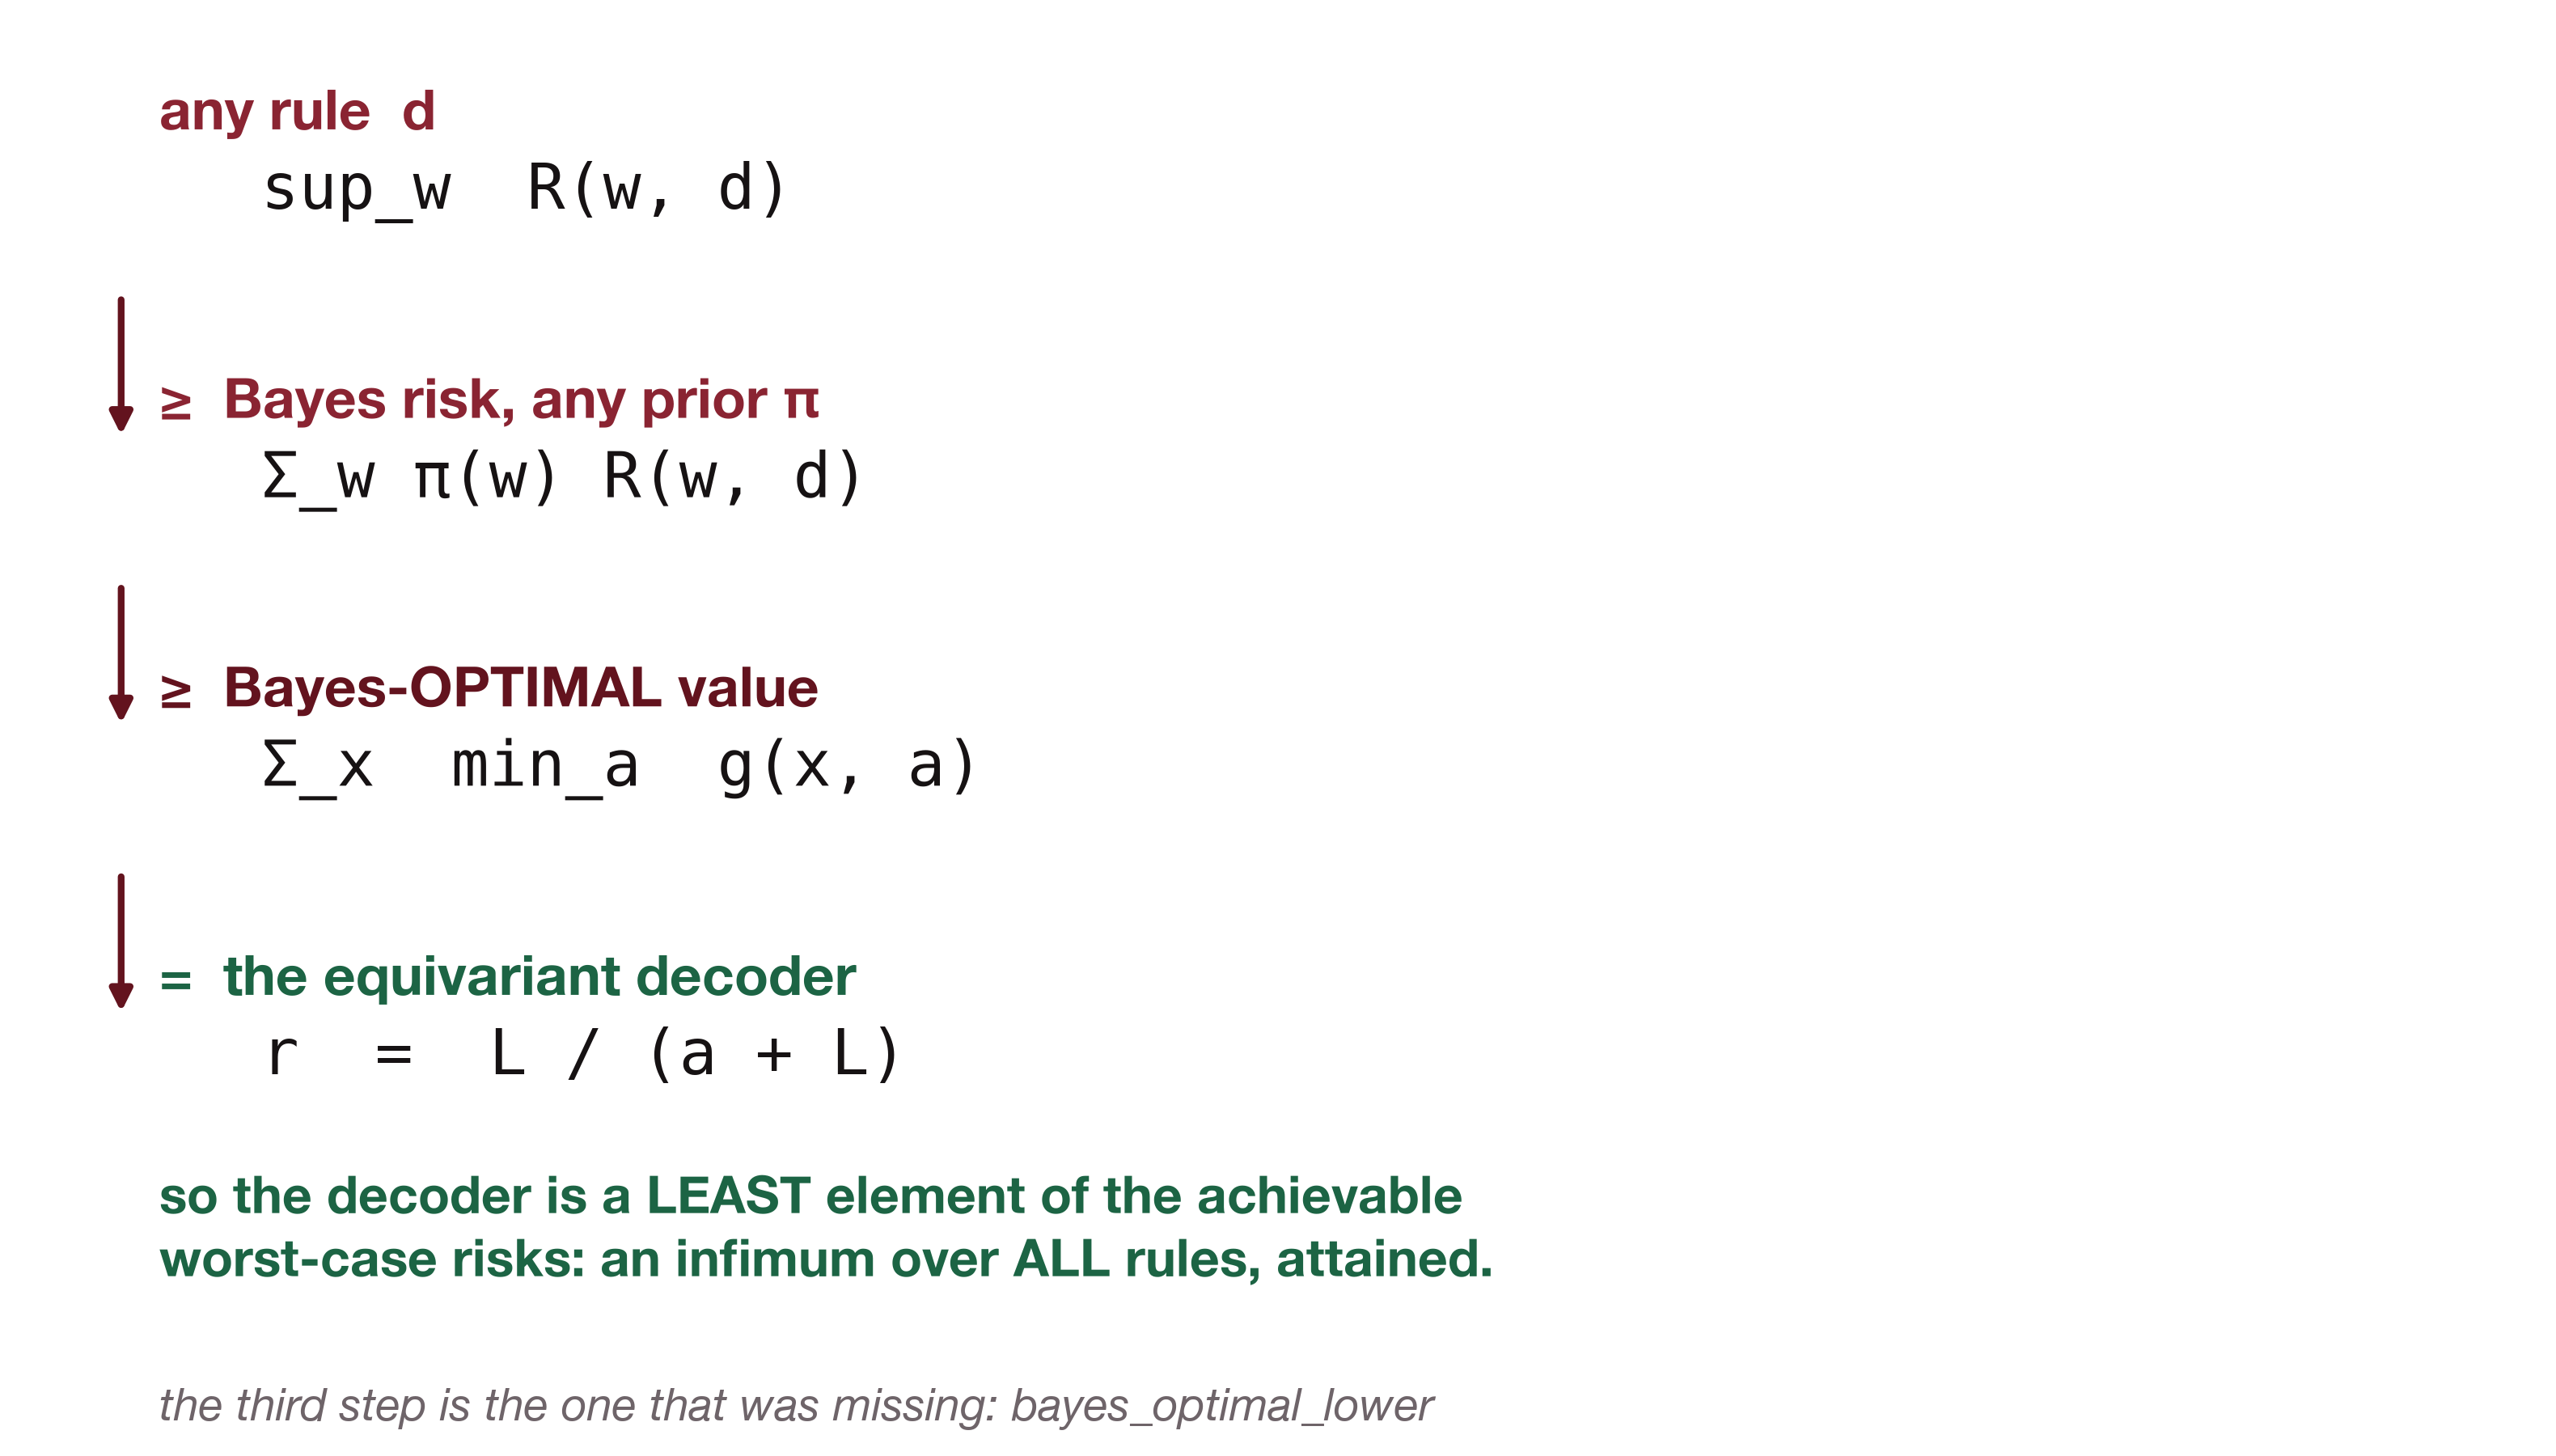
\includegraphics[width=\columnwidth]{support_fig2_minimax.png}
\caption{The minimax chain. Bayes risk factors through the posterior loss; the pointwise
minimum lower-bounds every rule and is attained; the worst case dominates the Bayes risk;
and the equivariant decoder's constant risk meets the resulting bound. The third step---
optimality over \emph{all} rules---is the one that was missing, and it is what turns
flatness into optimality.}
\label{fig:minimax}
\end{figure}

\section{What the chain needs, step by step}
\label{sec:chain}

The four statements of Sections~\ref{sec:bayes} and \ref{sec:minimax} compose into a single
conclusion, and it is worth setting out what each contributes, because three of the four are
textbook and the interest lies in which one was absent.

\emph{Factorisation} (Theorem~\ref{thm:factor}) is bookkeeping. It rewrites the Bayes risk
so that an arbitrary rule's dependence is separated observation by observation. It uses only
the exchange of two finite sums and would be true of any finite decision problem.

\emph{Pointwise optimality} (Theorem~\ref{thm:optimal}) is the step that was missing. It
converts the separated form into a bound valid for \emph{every} rule, by minimising each
summand independently, and it is the only place a quantifier over rules appears. Without it
the chain has no lower bound on anything but the specific decoder under study.

\emph{Attainment} (the second half of Theorem~\ref{thm:optimal}) upgrades the infimum to a
minimum. In a finite action set this is immediate, and its role is to let the conclusion be
stated as membership in the achievable set rather than as an unattained bound.

\emph{Domination} (the first inequality in Theorem~\ref{thm:minimax}) is the standard
observation that a weighted average is at most a supremum. It carries the Bayes bound to the
worst case, at the cost of fixing a prior---which is why the result is minimaxity through
one prior and not a general minimax theorem.

\subsection{Where the earlier statement stopped}

The earlier treatment had factorisation and domination, and it had the decoder's constant
risk as a hypothesis. From those it concluded that the decoder's worst case equals its
Bayes risk---true, and a statement about the decoder alone. The quantifier over rules never
appeared, so nothing followed about alternatives.

Adding Theorem~\ref{thm:optimal} changes the conclusion's subject from the decoder to the
problem. Adding Proposition~\ref{prop:symmetry} removes the constant-risk hypothesis. What
remains is a statement quantified over all rules with no hypotheses about the decoder, which
is what C2 and C3 claim.

\section{The decide--recover separation}
\label{sec:separation}

\begin{theorem}[Exact separation]
\label{thm:separation}
In the symmetric model the decide risk is
\begin{equation}
R_{\mathrm{dec}}\;=\;\frac{1}{2}(1-P)^{N}
\quad\text{exactly, flat in } K,
\label{eq:decide}
\end{equation}
while the number of samples needed for recovery grows like $K\log K$.
\end{theorem}

\begin{proof}[Proof outline]
The decide risk collapses to \eqref{eq:decide} by Theorem~\ref{thm:sampling} and the
equivariant form \eqref{eq:decoder}; the expression does not mention $K$ at all, because the
decision is correct as soon as the named tip is safe and that event's probability is
determined within a class. The recovery count is bounded below by a coupon-collector
argument over the $K$ classes.
\end{proof}

\leanbox{\lean{binary\_decide\_value}, \lean{decide\_upper\_expect},
\lean{growing\_K\_recover} in \lean{LeanSupportDecideRecoverV1}}

The comparison is therefore between an \emph{identity} and a growth rate, not between two
estimates. That is what ``exact separation'' means here and is stronger than the usual
asymptotic statement: the decide side is not bounded, it is computed.

\begin{figure}[htbp]
\centering
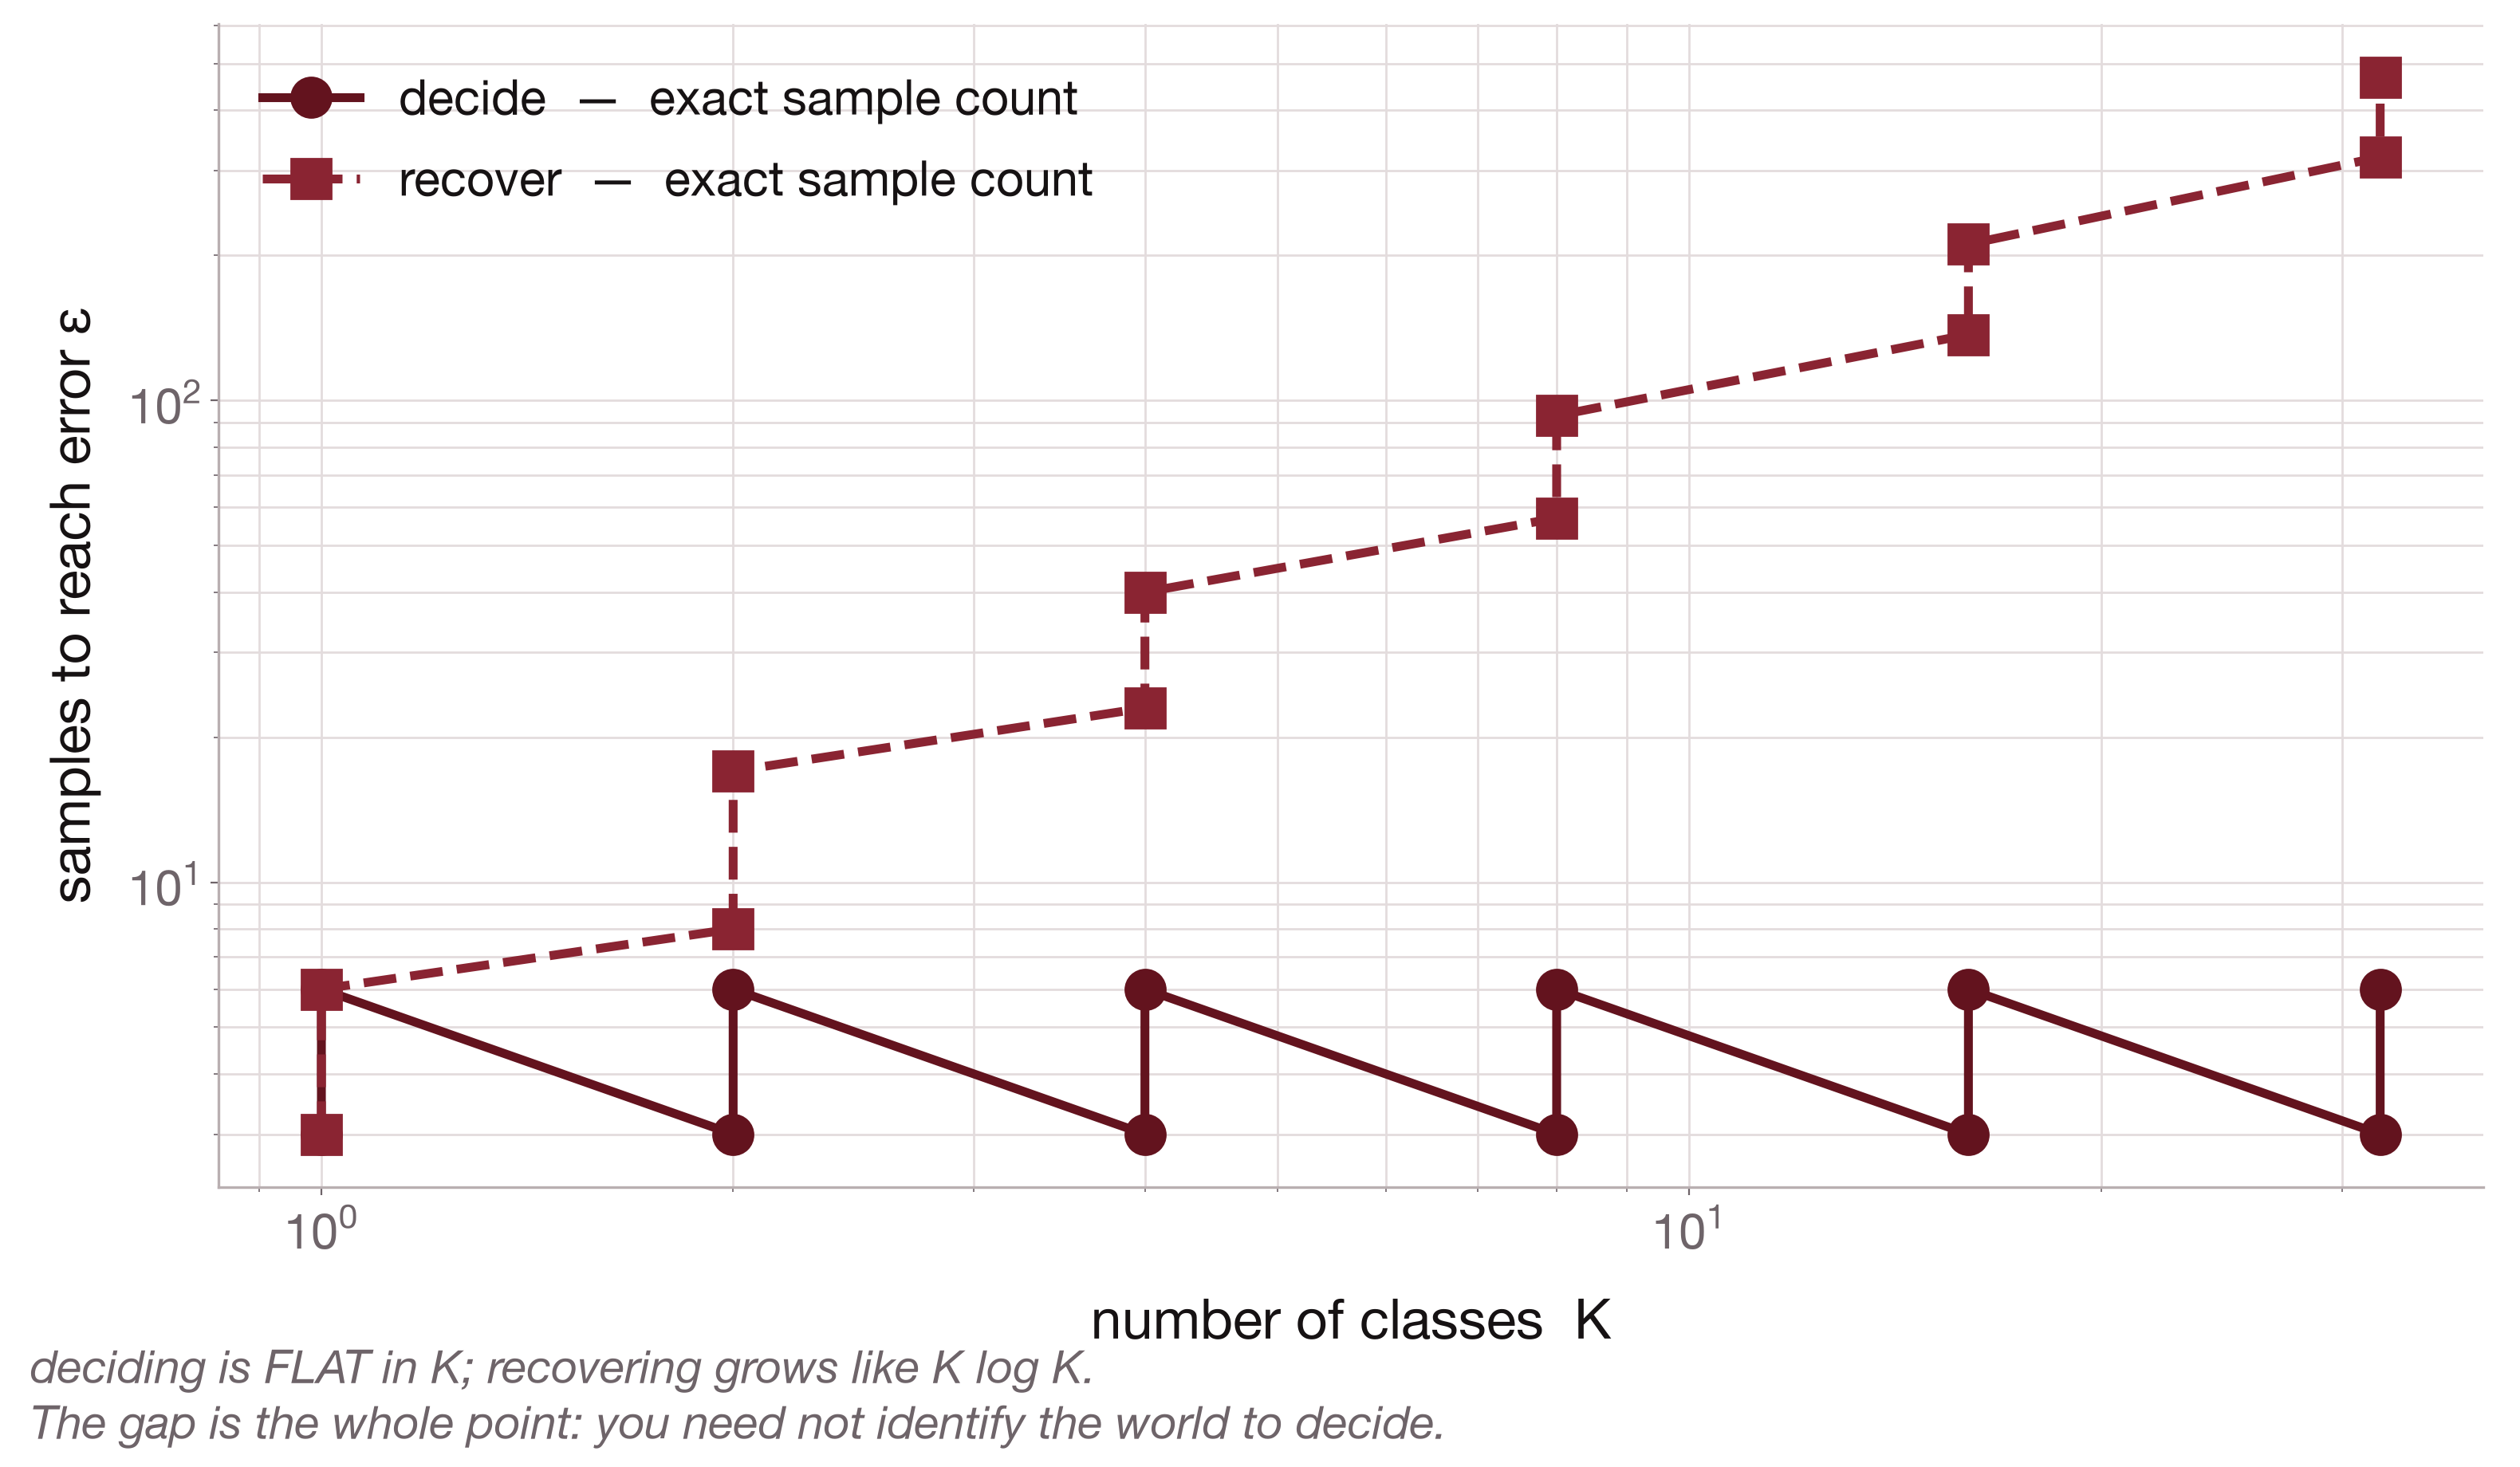
\includegraphics[width=\columnwidth]{support_fig1_separation.png}
\caption{Exact sample counts. Deciding is flat in the number of classes $K$; recovering
grows like $K\log K$. Both counts are exact integers computed from the closed forms rather
than simulated, so the widening gap is an identity against a growth rate.}
\label{fig:separation}
\end{figure}

\section{Reading the two costs}
\label{sec:reading}

Before the numbers, it is worth being precise about what each cost measures, since
``deciding'' and ``recovering'' are both informal until tied to an error criterion.

\emph{Deciding} means: after $N$ observations, name one tip and be wrong with probability at
most $\varepsilon$, where wrong means the named tip is unsafe. By
Theorem~\ref{thm:equivariant} the best achievable error at a transcript is
\eqref{eq:decoder}, and \eqref{eq:decide} is its value in the symmetric model, so the decide
cost is the least $N$ making that at most $\varepsilon$.

\emph{Recovering} means: after $N$ observations, report the world---the full unsafe set
across all classes---and be wrong with probability at most $\varepsilon$. The error event is
that some unsafe tip anywhere has gone unobserved, which is where the $K$-dependence enters:
every class must be resolved, and the probability that at least one is not is what
inclusion--exclusion computes.

\subsection{The comparison is between two thresholds, not two rates}

Both costs are defined as least $N$ meeting the same $\varepsilon$, so the comparison in
Table~\ref{tab:separation} is between two numbers computed the same way. This matters
because a comparison between, say, an exact decide cost and an asymptotic recovery rate
would be sensitive to the constant hidden in the rate; here both sides are exact integers
and the ratio is their quotient.

It also means the ratio is not scale-free. At $\varepsilon=\tfrac{1}{10}$ and $K=2$ the
ratio is $8/3\approx2.67$; at $\varepsilon=\tfrac{1}{100}$ it is $17/6\approx2.83$. The
ratio grows with $K$, which is the claim, and moves slightly with $\varepsilon$, which is
neither claimed nor surprising: the two costs have different $\varepsilon$-dependence, so
their quotient does too.

\section{Results}
\label{sec:results}

\subsection{Deciding is flat in $K$; recovering is not}

Across the parameter grid the exact decide count is independent of the number of classes
while the exact recovery count grows, and the ratio between them grows without bound as $K$
increases. Both counts are exact integers computed from the closed forms, not simulated.

The reason the decide count does not move is visible in \eqref{eq:decide}: $K$ does not
appear. A decision is correct as soon as the named tip is safe, and whether it is safe is
settled inside a single class; the other $K-1$ classes contribute nothing to the event. A
recovery, by contrast, must resolve every class, and the coupon-collector cost of doing so
is what grows.

\begin{table*}[t]
\caption{Exact sample counts for deciding and for recovering, on the model
$a_{i}=b_{i}=1$, $p_{i}=P/K$ with total unsafe mass $P$ held fixed. Every entry is exact
rational arithmetic; nothing is simulated. The decide column does not move with $K$---the
same count serves $K=1$ and $K=64$ at a given $(P,\varepsilon)$, which is
\eqref{eq:decide}---while the recover column grows, and with it the ratio. The last two
columns are the two risks evaluated at the \emph{decide} count, so they show directly what a
recovery-based procedure would still be carrying at the moment a decision is already safe.
The recovery law is an inclusion--exclusion identity and assumes no independence between
classes.}
\label{tab:separation}
\centering
\footnotesize
\setlength{\tabcolsep}{6pt}
\begin{tabular}{@{}rrrrrrrr@{}}
\toprule
$K$ & $P$ & $\varepsilon$ & $N_{\mathrm{decide}}$ & $N_{\mathrm{recover}}$ &
ratio & $R_{\mathrm{dec}}$ at $N_{\mathrm{decide}}$ & $R_{\mathrm{rec}}$ at $N_{\mathrm{decide}}$ \\
\midrule
1 & $\frac{1}{2}$ & $\frac{1}{10}$ & 3 & 3 & 1.000 & $\frac{1}{16}$ & $\frac{1}{16}$ \\
1 & $\frac{1}{2}$ & $\frac{1}{100}$ & 6 & 6 & 1.000 & $\frac{1}{128}$ & $\frac{1}{128}$ \\
2 & $\frac{1}{2}$ & $\frac{1}{10}$ & 3 & 8 & 2.667 & $\frac{1}{16}$ & $\frac{25}{64}$ \\
2 & $\frac{1}{2}$ & $\frac{1}{100}$ & 6 & 17 & 2.833 & $\frac{1}{128}$ & $\frac{713}{4096}$ \\
4 & $\frac{1}{2}$ & $\frac{1}{10}$ & 3 & 23 & 7.667 & $\frac{1}{16}$ & $\frac{841}{1024}$ \\
4 & $\frac{1}{2}$ & $\frac{1}{100}$ & 6 & 40 & 6.667 & $\frac{1}{128}$ & $\frac{345741}{524288}$ \\
8 & $\frac{1}{2}$ & $\frac{1}{10}$ & 3 & 57 & 19.000 & $\frac{1}{16}$ & $\frac{64741}{65536}$ \\
8 & $\frac{1}{2}$ & $\frac{1}{100}$ & 6 & 93 & 15.500 & $\frac{1}{128}$ & $\frac{260394461}{268435456}$ \\
16 & $\frac{1}{2}$ & $\frac{1}{10}$ & 3 & 137 & 45.667 & $\frac{1}{16}$ & $\frac{67105549}{67108864}$ \\
16 & $\frac{1}{2}$ & $\frac{1}{100}$ & 6 & 211 & 35.167 & $\frac{1}{128}$ & $\frac{2198711433501}{2199023255552}$ \\
32 & $\frac{1}{2}$ & $\frac{1}{10}$ & 3 & 320 & 106.667 & $\frac{1}{16}$ & $\frac{17592186030877}{17592186044416}$ \\
32 & $\frac{1}{2}$ & $\frac{1}{100}$ & 6 & 469 & 78.167 & $\frac{1}{128}$ & $\frac{4611686007394094621}{4611686018427387904}$ \\
\bottomrule
\end{tabular}
\end{table*}


Table~\ref{tab:separation} gives the exact counts on the model $a_{i}=b_{i}=1$,
$p_{i}=P/K$ with the total unsafe mass $P$ held fixed. At $P=\tfrac12$,
$\varepsilon=\tfrac{1}{100}$, deciding takes $6$ samples whether there is one class or
thirty-two, while recovering takes $6$, $17$, and more as $K$ grows. The ratio is not a
fitted slope: both columns are exact integers obtained by inverting closed forms in rational
arithmetic.

The last two columns say the same thing from the risk side. At the moment the decide risk
has reached $\tfrac{1}{128}$, the recovery risk is still $\tfrac{713}{4096}$ at $K=2$---
about twenty-two times larger---and the gap widens with $K$. An experimenter who stops when
they can decide is done; one who stops when they can identify is still far from it.

\subsection{The recovery law makes no independence assumption}

It is worth recording how the recovery side is computed, because an independence assumption
would weaken the comparison. The probability that recovery is incomplete is obtained by
inclusion--exclusion over the classes,
\begin{equation}
R_{\mathrm{rec}}
\;=\;1-\sum_{k}\binom{K}{k}\Bigl(-\tfrac12\Bigr)^{k}
     \Bigl(1-\tfrac{kP}{K}\Bigr)^{N},
\end{equation}
which is an identity, not a bound, and assumes nothing about how the classes interact. The
same quantity is sandwiched between $\tfrac12\Pr(U>0)$ and $\Pr(U>0)$, verified exactly at
several $N$, which is what allows the coupon-collector \emph{scale} to be quoted for
comparison without being relied on.

That distinction is maintained in the artifact and is repeated here: the coupon-collector
constant is not proved, and the column labelled with that scale is for comparison only. The
growth claim rests on the exact counts.

\subsection{The decoder is optimal, not merely flat}

With Theorem~\ref{thm:minimax} the equivariant decoder is a least element of the achievable
worst-case risks, so no decision rule whatsoever---randomised or not, adaptive or not---
achieves a smaller worst case on this problem. The quantifier is over all maps from
observations to actions, which in a finite setting is every rule there is.

\section{A worked instance}
\label{sec:worked}

The abstract chain is easier to check against a small case, so we record one.

Take $a=3$ safe tips and $b=2$ unsafe tips, so $|T|=5$. Before any observation the
transcript is empty, $L=b-0=2$, and \eqref{eq:decoder} gives risk
$r=\tfrac{2}{3+2}=\tfrac25$: naming a tip at random is wrong two times in five, which is
just the unsafe fraction.

Suppose one unsafe tip is revealed, $|R|=1$. Then $L=1$ and $r=\tfrac{1}{3+1}=\tfrac14$.
Note what has and has not been learned. The world is \emph{not} identified: the remaining
unsafe tip could be any of the four unexplored ones, so $\binom{4}{1}=4$ worlds remain
compatible. But the risk is the same in all four, because each has exactly one unsafe tip
among four unexplored---this is Lemma~\ref{lem:hidden}, and it is why
Theorem~\ref{thm:equivariant} can speak of ``the'' conditional risk at a transcript.

Reveal the second unsafe tip and $L=0$, so $r=0$: every unexplored tip is safe and the
decoder cannot err. The world \emph{is} now identified, but only incidentally---the risk
reached zero because $L$ did, not because the world became known, and at $|R|=1$ the risk
was already $\tfrac14$ with four worlds still in play.

\subsection{The same instance through the minimax chain}

Fix any prior $\pi$ on the $\binom{5}{2}=10$ worlds that is invariant under relabelling the
tips. Theorem~\ref{thm:factor} writes the Bayes risk of an arbitrary rule as a sum over
transcripts of $g(x,d(x))$. At a transcript with $|R|=1$, the posterior is uniform over the
four compatible worlds by symmetry, so $g(x,a)$ is $\pi$-weight times $\tfrac14$ for a tip
that is unsafe in one of the four and $0$ for one that is safe in all---and there is no such
tip, since each unexplored tip is unsafe in exactly one compatible world. Hence
$\min_{a}g(x,a)$ is attained at every unexplored tip equally, and the Bayes-optimal value at
that transcript equals the equivariant decoder's $\tfrac14$.

Summing over transcripts, the Bayes-optimal value equals the decoder's constant risk, which
by Theorem~\ref{thm:minimax} makes it a least element of the achievable worst-case risks.
The instance also shows why Theorem~\ref{thm:optimal}'s attainment clause matters: the
argmin is not unique here---every unexplored tip attains it---and the theorem needs only
that \emph{some} choice exists, which finiteness supplies.

\section{Why the decoder is the natural one}
\label{sec:natural}

Theorem~\ref{thm:minimax} says the equivariant decoder is optimal. It does not explain why
that decoder, of all rules, is the one that meets the bound, and the explanation is short
enough to give.

\subsection{Symmetry forces the form}

Fix a relabelling-invariant prior. The posterior at a transcript $R$ is uniform over the
compatible worlds by symmetry, and by Lemma~\ref{lem:hidden} each compatible world has
exactly $L$ unsafe tips among the $a+L$ unexplored ones. Summing over compatible worlds,
each unexplored tip is unsafe in the same number of them, so the posterior probability that
a given unexplored tip is unsafe is $L/(a+L)$, identically for every unexplored tip.

The posterior loss $g(x,a)$ of Theorem~\ref{thm:factor} is therefore \emph{constant} across
unexplored tips, and strictly larger for explored ones---which are known to be unsafe. Every
unexplored tip is thus an argmin, and every rule naming some unexplored tip is Bayes-optimal
at that transcript. The uniform decoder is one such rule.

\subsection{So optimality is shared, and that is informative}

An immediate consequence is that the equivariant decoder is not \emph{uniquely} optimal:
naming the lowest-indexed unexplored tip is equally optimal, as is any other selection rule
among unexplored tips. What all optimal rules share is the constraint---never name an
explored tip---and the freedom is in which unexplored one.

This is worth stating because it identifies what the result actually rules out. It does not
say randomisation helps; it does not say the uniform choice is special. It says that the
information in the transcript is exhausted by the set of explored tips, that no further
structure in the transcript can be exploited, and that any rule respecting the one
constraint attains the minimax value. A rule that tried to be cleverer---weighting
unexplored tips by some heuristic---cannot do better, because there is nothing left to be
clever about.

\subsection{Where the symmetry would fail}

The argument above uses the relabelling invariance of the prior twice: to make the posterior
uniform over compatible worlds, and to make each unexplored tip equally likely to be unsafe.
With an asymmetric prior---one that believes certain tips are more often unsafe---neither
step survives, the posterior loss varies across unexplored tips, and the argmin rule is no
longer the uniform one. Theorems~\ref{thm:factor} and \ref{thm:optimal} still hold, since
they assume nothing about the prior; what fails is the identification of the argmin with the
uniform decoder, and hence Theorem~\ref{thm:minimax}'s conclusion about \emph{that} decoder.

The paper's scope section records the fixed prior for this reason. The minimax chain is
general; the decoder that meets its bound is the one symmetry selects.

\section{Formal verification}
\label{sec:verification}

Every theorem above is machine-checked in Lean~4, toolchain
\texttt{leanprover/lean4:v4.34.0-rc2} against mathlib revision \texttt{1f495c61}.

\subsection{Acceptance contract}

A module counts as accepted only when all six of the following hold: the compiler exits zero
with no errors; the source hash is unchanged \emph{across} the compile; the compiled
artifact is newer than its source; at least one \texttt{\#print axioms} directive is
present; the axiom set of every audited declaration lies within
$\{\textsf{propext},\textsf{Classical.choice},\textsf{Quot.sound}\}$; and no \texttt{sorry}
appears anywhere in the file.

\subsection{The crux statements as they are checked}

\begin{figure}[htbp]
\footnotesize
\hrule\vspace{4pt}
\begin{tabbing}
\quad\=\quad\=\kill
\lean{theorem bayes\_optimal\_lower} \\
\> \lean{(pri : World $\to$ $\mathbb{R}$) (P : World $\to$ Obs $\to$ $\mathbb{R}$)} \\
\> \lean{(L : World $\to$ Act $\to$ $\mathbb{R}$) (d : Obs $\to$ Act) :} \\
\> \lean{bayesOptValue pri P L $\le$ bayesRisk pri P L d} \\[6pt]
\lean{theorem equivariant\_is\_minimax [Nonempty World]} \\
\> \lean{(pri : World $\to$ $\mathbb{R}$) (P : World $\to$ Obs $\to$ $\mathbb{R}$)} \\
\> \lean{(L : World $\to$ Act $\to$ $\mathbb{R}$)} \\
\> \lean{(hpi : $\forall$ w, 0 $\le$ pri w) (hsum : $\sum$ w, pri w = 1)} \\
\> \lean{(d$_0$ : Obs $\to$ Act) (r : $\mathbb{R}$)} \\
\> \lean{(hconst : $\forall$ w, risk P L d$_0$ w = r)} \\
\> \lean{(hopt : bayesOptValue pri P L = r) :} \\
\> \lean{IsLeast \{v | $\exists$ d : Obs $\to$ Act,} \\
\> \qquad\lean{univ.sup' univ\_nonempty (risk P L d) = v\} r}
\end{tabbing}
\vspace{-4pt}\hrule
\caption{The optimality step and the conclusion, as checked. In
\lean{bayes\_optimal\_lower} the rule \lean{d} is an \emph{arbitrary} function
\lean{Obs $\to$ Act}: nothing restricts it, since in a finite setting every rule is such a
function. The conclusion of \lean{equivariant\_is\_minimax} is \lean{IsLeast}---the value is
both a lower bound on the achievable worst-case risks and a member of that set, which is the
difference between ``no rule is known to do better'' and ``no rule does better''. Its two
hypotheses \lean{hconst} and \lean{hopt} are what the surrounding sections supply:
Theorem~\ref{thm:equivariant} with Proposition~\ref{prop:symmetry} gives the first, and the
posterior computation of Section~\ref{sec:natural} gives the second.}
\label{fig:statements}
\end{figure}

The choice of \lean{IsLeast} is deliberate and is the formal expression of what was missing
before. A lower-bound statement alone would say the worst-case risk of every rule is at
least $r$; membership says $r$ is achieved, and by a rule with constant risk. Together they
say the decoder is optimal rather than merely unimprovable-as-far-as-we-know.

The hypothesis \lean{[Nonempty World]}, together with the finiteness of the action set that
Theorem~\ref{thm:optimal}'s existence clause needs, is where that theorem enters. Without a
non-empty action set the pointwise minimum is over an empty family and the statement is
vacuous; with it, the argmin rule exists and the infimum is attained.

\subsection{Evidence per step}

\begin{table}[htbp]
\caption{Evidence per step. All cited declarations are axiom-audited.}
\label{tab:inventory}
\centering
\footnotesize
\setlength{\tabcolsep}{3pt}
\begin{tabular}{@{}llr@{}}
\toprule
Step & Module & Aud. \\
\midrule
Sampling, Thm~\ref{thm:sampling}      & \lean{LeanSupportSamplingLawV1}        & 9 \\
Decoder, Thm~\ref{thm:equivariant}    & \lean{LeanSupportEquivariantDecoderV1} & 4 \\
Factorisation, Thm~\ref{thm:factor}   & \lean{LeanSupportMinimaxLowerV1}       & 6 \\
Optimality, Thm~\ref{thm:optimal}     & \lean{LeanSupportMinimaxLowerV1}       & 6 \\
Minimax, Thm~\ref{thm:minimax}        & \lean{LeanSupportMinimaxLowerV1}       & 6 \\
Symmetry, Prop~\ref{prop:symmetry}    & \lean{LeanSupportMinimaxLowerV1}       & 6 \\
Separation, Thm~\ref{thm:separation}  & \lean{LeanSupportDecideRecoverV1}      & 11 \\
\bottomrule
\end{tabular}
\end{table}

\subsection{Reproducing the counts}

Table~\ref{tab:separation} is produced by inverting two closed forms in exact rational
arithmetic. For each $(K,P,\varepsilon)$ the decide count is the least $N$ with
$\tfrac12(1-P)^{N}\le\varepsilon$, computed by incrementing $N$ over exact rationals rather
than by taking a logarithm and rounding---the logarithmic expression is reported alongside as
\emph{scale} and is not used to produce the integer. The recover count is the least $N$ with
the inclusion--exclusion expression at most $\varepsilon$, computed the same way.

Two consequences follow from doing it this way. The integers in the table are the true
thresholds, not rounded approximations, so a claim that deciding needs exactly $6$ samples
at $(P,\varepsilon)=(\tfrac12,\tfrac{1}{100})$ is exact. And the risks in the last two
columns are exact rationals---$\tfrac{1}{128}$ and $\tfrac{713}{4096}$---rather than decimal
approximations, which is what makes the twenty-two-fold gap at $K=2$ a computed quantity
rather than a rounded one.

The grid is $K\in\{1,2,4,8,16,32\}$ and $\varepsilon\in\{\tfrac{1}{10},\tfrac{1}{100}\}$ at
$P=\tfrac12$, twelve rows in all. Extending it is cheap but adds nothing: the decide column
is constant in $K$ by \eqref{eq:decide}, which is a theorem, and the table's role is to show
the recover column moving against it.

\subsection{Scope of the formalisation}

The displayed results are the load-bearing chain, not the corpus. The Support strand
contains $50$ Lean source files with $870$ theorem and lemma statements, of which $21$
modules carry an acceptance receipt covering $184$ declarations whose axiom set was printed
and checked. Across the programme of which this paper is one part: $762$ files, $7{,}199$
statements, $108$ accepted modules, $860$ audited declarations.

No module cited in this paper contains a \texttt{sorry}. Seven occurrences exist in the
wider repository, in audit scaffolding and in files named as conjectures; the overlap
between the cited set and the files containing them was computed and is empty.

\subsection{What formalisation caught}

Two formulations were withdrawn under the prover, and the first is the reason this paper
exists.

The original minimax statement was of the form: if the decoder's risk is constant, then its
worst case equals its Bayes risk. Written out in Lean, the hypothesis
\lean{hconst} appeared as a premise and no quantifier over rules appeared anywhere in the
statement. Reading it back made the gap unmissable---the conclusion mentions one rule and
one prior, and there is no second rule in the statement to compare against. The prose
summary had described this as ``the decoder is minimax'', which the statement does not say.

The second was in the sampling law. An early version of Theorem~\ref{thm:sampling} assumed
independence between classes in order to factor the expectation of a product of indicators.
The assumption is unnecessary: the expectation of a sum of indicators factors by linearity,
and the quantity actually needed is a sum. Removing the assumption also removed a hypothesis
from the recovery law, which is why the inclusion--exclusion identity quoted in
Section~\ref{sec:results} carries no independence condition.

Neither correction changes a number in Table~\ref{tab:separation}. Both change what the
theorems entitle one to say, which is the category of defect a numerical check cannot find.

\section{Generalising the argument}
\label{sec:general}

Two of the results are specific to this problem and two are not, and separating them says
where the paper's technique applies.

\subsection{What generalises}

Theorems~\ref{thm:factor} and \ref{thm:optimal} use nothing about the problem beyond
finiteness of the world, observation and action sets. Any decision problem with those
properties admits the same factorisation and the same pointwise-minimisation bound, and in
any such problem the infimum over rules is attained. The recipe for establishing minimaxity
is therefore: find a prior, compute the Bayes-optimal value, exhibit a rule with constant
risk equal to it, and conclude \lean{IsLeast}. Each of the four steps is mechanical except
the third.

Proposition~\ref{prop:symmetry} likewise needs only a transitive group action on worlds
under which the risk is invariant. Where a problem has such symmetry, the constant-risk step
comes free, which is what makes the recipe usable in practice: exhibiting a rule with
constant risk is hard in general and immediate under transitivity.

\subsection{What does not}

Theorem~\ref{thm:equivariant} uses the specific structure that compatibility forces
$R\subseteq W$ with $|W|=b$ fixed. An observation process that revealed partial information
about safe tips, or one in which $|W|$ were unknown, would break
Lemma~\ref{lem:hidden}---the hidden count would vary across compatible worlds---and the
conditional risk would depend on the world after all.

Theorem~\ref{thm:separation} uses the symmetric model with $a_{i}=b_{i}=1$ and total unsafe
mass held fixed. Both the flatness in $K$ and the inclusion--exclusion form of the recovery
law come from it, and neither is claimed outside it.

\subsection{The transferable observation}

Stripped of the model, the paper's content is this: when the quantity to be reported is a
decision rather than a parameter, the cost may not scale with the parameter's complexity,
and whether it does is settled by asking what the posterior loss depends on. Here it depends
on $|R|$ alone, so the cost is flat in $K$. In another problem it might depend on more, and
the same computation would say so. The technique is the computation, not the answer.

\section{Discussion}
\label{sec:discussion}

\subsection{The gap, and why it was worth closing}

The gap closed here is small to state and large in consequence. A constant-risk decoder is
not automatically a good one: constancy is a property of the decoder, optimality is a
property of the problem. Without an infimum over rules, the earlier statement was compatible
with every rule being bad, including this one.

Theorem~\ref{thm:optimal} supplies that infimum, and because the action set is finite the
infimum is attained, so the argument needs no compactness and no limit. This is a
structural simplification worth noting: in a continuous action space the pointwise minimum
may fail to be attained and the least-element conclusion would have to be weakened to an
infimum, with a corresponding weakening of what ``no rule does better'' means.

\subsection{Why flatness and optimality are independent}

The distinction the paper turns on is worth an explicit example, since ``constant risk''
sounds like a strong property.

Consider the rule that always names the first tip in some fixed enumeration of $T$,
regardless of the transcript. Under a relabelling-invariant prior its risk is the same in
every world---perfectly flat---and it is $b/(a+b)$, the unconditional unsafe fraction, at
\emph{every} transcript. It never improves, because it ignores the data. So it is flat and,
after even one observation, strictly worse than the equivariant decoder.

Flatness therefore rules nothing out. What the earlier treatment established was that the
equivariant decoder is in the same category as this trivial rule with respect to
world-dependence, which is a real property---it means the decoder has no adversarial world
---but says nothing about how it compares to other rules. The infimum of
Theorem~\ref{thm:optimal} is what supplies the comparison, and
Proposition~\ref{prop:symmetry} then lets the flatness be derived rather than assumed, so
the two properties are established in the right order: optimality from the infimum, flatness
from symmetry, and the conjunction from the fact that the decoder's constant value meets the
bound.

\subsection{The practical reading}

An experimenter facing many classes should not pay for identification. The cost of naming a
safe tip does not grow with the number of classes; the cost of learning which world one is
in does, and by Theorem~\ref{thm:separation} the gap between the two is unbounded in $K$.

The corollary for system design is that the question ``what do I need to know?'' should be
asked before ``how do I learn it?''. If the downstream decision is a choice among actions
rather than a report of the parameter, the identification cost may be entirely avoidable,
and Theorem~\ref{thm:minimax} says the avoidance is not a heuristic---the decoder that
ignores identification is optimal.

\subsection{Two objections answered}

\emph{``Minimaxity through one prior is weaker than a minimax theorem.''} Correct, and the
scope section says so. What is obtained is a value $v$ that lower-bounds the worst-case risk
of every rule and is achieved by one, which is exactly the definition of a minimax-optimal
rule; what is \emph{not} obtained is a saddle point, i.e.\ a prior that is least favourable
in the game-theoretic sense. The distinction matters if one wants to characterise the
least-favourable prior, and does not matter for the claim made, which is about rules rather
than priors. The prior used is any relabelling-invariant one, and
Section~\ref{sec:natural} shows all of them give the same Bayes-optimal value here.

\emph{``Finiteness makes the result easy.''} Also correct, and it is stated rather than
hidden. Attainment of the pointwise minimum is immediate in a finite action set, and with an
infinite one the conclusion would weaken from \lean{IsLeast} to an infimum that may not be
achieved. But the ease is in the \emph{proof}, not in the \emph{statement}: the earlier
treatment had the same finite setting and did not have the result, because the missing
ingredient was the quantifier over rules rather than a technical difficulty in handling it.
That is the paper's actual point---the gap was one of formulation, and finiteness is why
closing it cost a page rather than a chapter.

\subsection{What is not established}

\begin{enumerate}
\item \textbf{One prior, not a minimax theorem.} The prior is arbitrary but \emph{fixed}:
this is minimaxity through one Bayes prior, not a general minimax theorem, and no saddle
point is claimed in the abstract.

\item \textbf{Everything is finite.} Worlds, transcripts and actions are finite throughout,
and nothing extends to infinite action sets where the pointwise minimum may fail to be
attained.

\item \textbf{Transitivity is a hypothesis.} The transitivity of the relabelling group is
supplied where it is used. It is a fact about this problem rather than a theorem proved in
general.

\item \textbf{The observation process is given.} Nothing here designs the sampling; the
analysis begins from a completed transcript.
\end{enumerate}

\subsection{What the separation does not say}

Theorem~\ref{thm:separation} compares the cost of deciding against the cost of recovering
\emph{on this model}: $a_{i}=b_{i}=1$ per class, total unsafe mass $P$ held fixed as $K$
grows. Three readings it does not support are worth naming.

It does not say identification is never worth its cost. If the downstream use of the
transcript is something other than naming one safe tip---predicting future observations,
say, or acting repeatedly---the decision problem is different and the separation says
nothing about it.

It does not say the decide cost is independent of everything. It is independent of $K$,
which is the point, but it depends on $P$ and $\varepsilon$ through \eqref{eq:decide} in the
usual way. Table~\ref{tab:separation} shows the dependence on $\varepsilon$ directly: at
$P=\tfrac12$ the count rises from $3$ to $6$ as $\varepsilon$ falls from $\tfrac{1}{10}$ to
$\tfrac{1}{100}$.

And it does not extend the fixed-$K$ constants. The model here has $a_{i}=b_{i}=1$; the
constants appearing in the fixed-$K$ analysis depend on $K$ and are not covered, as the
artifact's own scope note records.

\subsection{Open problems}

Whether the least-element conclusion survives an infinite action set, with the pointwise
minimum replaced by an infimum and attainment recovered under a compactness hypothesis, is
the first question. Whether the flatness of \eqref{eq:decide} in $K$ survives asymmetric
classes---where the safe/unsafe split differs between classes, so the relabelling group is
no longer transitive---is the second, and Proposition~\ref{prop:symmetry} is exactly what
would fail. Third, the separation compares an exact decide cost against a coupon-collector
lower bound on recovery; an exact recovery cost would make the comparison an identity on
both sides.

\section{Conclusion}

The natural decoder---name a tip uniformly from the unexplored set---is not merely
convenient. Its risk is a function of the transcript alone, and it is a least element of the
worst-case risks achievable by \emph{any} decision rule. Deciding costs a number that does
not grow with the number of classes, while identifying the world does, so the two problems
are separated exactly and not merely asymptotically.

The general lesson is about what to prove rather than what to build. The decoder here was
never in doubt as a practical choice---it is what anyone would implement. What was in doubt
was whether implementing it was a compromise, and answering that took a quantifier over all
rules rather than a better decoder. Where a practical choice is obvious, the useful
theoretical work is often not to improve it but to establish that it cannot be improved, and
that work has a characteristic shape: a factorisation, a pointwise minimisation, and an
existence argument for the minimiser.

\section*{Acknowledgment}

The formal development uses the Lean~4 theorem prover and the mathlib library.

\begin{thebibliography}{00}

\bibitem{javdani2014} S. Javdani, Y. Chen, A. Karbasi, A. Krause, J. A. Bagnell, and
S. Srinivasa, ``Near-optimal Bayesian active learning for decision making,'' in
\emph{Proc. 17th Int. Conf. Artificial Intelligence and Statistics (AISTATS)}, 2014.

\bibitem{lehmann1998} E. L. Lehmann and G. Casella, \emph{Theory of Point Estimation},
2nd ed. New York, NY: Springer, 1998.

\bibitem{mathlib2020} The mathlib Community, ``The Lean mathematical library,'' in
\emph{Proc. 9th ACM SIGPLAN Int. Conf. Certified Programs and Proofs (CPP)}, 2020,
pp.~367--381.

\bibitem{demoura2021} L. de Moura and S. Ullrich, ``The Lean 4 theorem prover and
programming language,'' in \emph{Proc. 28th Int. Conf. Automated Deduction (CADE)}, 2021,
pp.~625--635.

\bibitem{wald1950} A. Wald, \emph{Statistical Decision Functions}. New York, NY: Wiley,
1950.

\bibitem{golovin2011} D. Golovin and A. Krause, ``Adaptive submodularity: Theory and
applications in active learning and stochastic optimization,'' \emph{J. Artif. Intell.
Res.}, vol.~42, pp.~427--486, 2011.

\bibitem{motwani1995} R. Motwani and P. Raghavan, \emph{Randomized Algorithms}. Cambridge,
U.K.: Cambridge Univ. Press, 1995.

\end{thebibliography}

\end{document}
